%
%
%   S A I J O
%
%

% created by kadono 2018/11/24 18:00
% edited by nakayama 2018/11/24 19:30

\documentclass[11pt,b5paper,papersize,dvipdfmx]{jsbook}

\usepackage{vuccaken}
\usepackage{vuccaken2018}
\usepackage{15saijo}

% 以下本文
\begin{document}
% \tableofcontents

% - - - - - - - - - - - - - - - - - - - - - - -
\kaishititle{人工衛星なんてもういいですから。}%
                {機械工学科1回生}{西條晴幸}
% - - - - - - - - - - - - - - - - - - - - - - -

%
\section*{はじめに}
この文章たちは私が4年ほど前に行った活動を基にしたものであるので、少々古い内容もありますが内容的には高校物理だけ(中学生でも少し勉強すれば読める…はず)なので、そこのあなたもさらっと読んでいってみてください。わからなかったらこの機会(?)に物理の「力学」と数学の「ベクトル」をちょちょいと勉強してみましょう。いざ。

\section{目的}
宇宙空間において,ある天体のまわりで初速度をもった物体を放つと,天体の重力と物体の運動から起きる慣性力(遠心力)が釣り合うことで,物体が天体のまわりを半永久的に周回する場合がある。この時の天体に対する物体の速度を第一宇宙速度と言う。地球における第一宇宙速度をBASIC言語のプログラムを用いて,物体の運動シミュレーションを行うことで概算する。
\section{手法}
\subsection{基本方程式}
原点$O$に質量$M$の恒星があり、位置$\vec{r}=(x,y)$に質量$m$の惑星が存在するとき、万有引力の法則を仮定すると、惑星の受ける力は距離の2乗に反比例する大きさと、惑星から恒星へと向かう向きを持っているので次のように書くことができる。
\begin{align}
    \vec{F} = -\frac{\vec r}{|\vec{r}|}\frac{GMm}{|\vec{r}|^2}
    \label{eq:sj-banyu}
\end{align}
ここで、$G$は万有引力定数である。\par
また、運動方程式により加速度$\vec{a}$は、力 $\vec{F}$によって次のように定められる。
\begin{align}
    \vec{a} = \frac{\vec{F}}{m}
    \label{eq:sj-undou}
\end{align}
そして、時刻$t$と$t+dt$の間の位置と速度の単位時間あたりの変化は、それぞれ平均の速度と平均の加速度と呼ばれる。
\begin{align}
    \frac{\vec{r}(t+dt) - \vec{r}(t)}{dt} = \vec{\overline{v}},
    \qquad
    \frac{\vec{v}(t+dt) - \vec{v}(t)}{dt} = \vec{\overline{a}}
\end{align}
ここで、平均の速度と加速度をそれぞれ時刻tでの速度と加速度で近似すれば、
\begin{align}
    \vec{r}(t+dt) \fallingdotseq \vec{r}(t) + \vec{\overline{v}}(t)dt,
    \qquad
    \vec{v}(t+dt) \fallingdotseq \vec{v}(t) + \vec{\overline{a}}(t)dt
\end{align}
となる。この式を成分で表せば、
\begin{align}
    \begin{split}
        x(t+dt) &\fallingdotseq x(t) + v_x(t)dt\\
        y(t+dt) &\fallingdotseq y(t) + v_y(t)dt\\
        v_x(t+dt) &\fallingdotseq v_x(t) + a_x(t)dt\\
        v_y(t+dt) &\fallingdotseq v_y(t) + a_y(t)dt
    \end{split}
    \label{eq:sj-seibun}
\end{align}
となり、ここでの加速度$a_x,a_y$は(\ref{eq:sj-banyu}),\,(\ref{eq:sj-undou})式より、
\begin{align}
\begin{split}
a_x(t) &= \frac{-x}{\sqrt{x^2+y^2}}\cdot \frac{GM}{(\sqrt{x^2+y^2})^2} = -x(x^2+y^2)^{-\frac{3}{2}}GM\\
a_y(t) &= \frac{-y}{\sqrt{x^2+y^2}}\cdot \frac{GM}{(\sqrt{x^2+y^2})^2} = -y(x^2+y^2)^{-\frac{3}{2}}GM
\end{split}
\label{eq:sj-kasoku}
\end{align}
と表すことができる。これら(\ref{eq:sj-seibun}),\,(\ref{eq:sj-kasoku})式を逐次解くことで位置と速度の時間発展を追うことができる。なお、恒星の質量は惑星に比べて十分大きく、その位置は変化しないとみなせるものとした。

%
\subsection{計算手法}
本研究の数値計算には、"Excel VBA"を用いた。万有引力定数のため、$G=6.67\times 10^{20}$、地球質量(ここから前項の”恒星”=地球とする)のため、$M=6\times 10^{24}$とした。時間の刻み$dt=0.001$として次の初期条件の下、時刻$t=25000$まで計算し、その間の位置、速度を出力した。
また、地球半径($r$)を概数で$6371\ \mathrm{km}$と仮定した。そして海抜$0.001\ \mathrm{km}$から直径に対して垂直に物体を打ち出し、地表に衝突することなく周回を続ける最低速度を求める(暇なので手打ちで有効数字5つほど)こととする。正確に第一宇宙速度を求める際には海抜$0\ \mathrm{km}$を用いるべきだが、$0\ \mathrm{km}$を用いると最初の地点で地表に衝突してしまうため、$0.001\ \mathrm{km}$とした。
\begin{table}[htb]
    \centering
    \caption{計算の初期条件}
    \begin{tabular}{c|cccc}
        変数 & \shortstack{\\$x$\\(物体の$x$座標)}& \shortstack{\\$y$\\(同$y$座標)} & \shortstack{\\$v_x$\\(速度の$x$成分)} & \shortstack{\\$v_y$\\(同$y$成分)} \\\hline
        初期条件 & 6371.001 & 0 & 0 & $V_y$
    \end{tabular}
    \label{tbl:sj-meex}
\end{table}
$V_y$を徐々に変化(手打ち)させていき、衝突しない最低速度を求める。\par
実際に使用したプログラムは付録Aに収録した。

% - - - - - - - -
\section{結果}
% - - - - - - - -
この計算によって次の結果が得られた。\par
\begin{table}[H]
    \centering
    \caption{各時刻における物体の位置と速度}
        \begin{tabular}{c|cccc}
            \hline
            時刻        &$x$座標     &$y$座標    &$x$速度   &$y$速度\\\hline
            0	        &6371.001	&0	        &0	        &7.9417\\
            1.000991	&6371.001	&7.957604	&-0.00988	&7.9417\\
            2.000037	&6371.001	&15.89091	&-0.01973	&7.9417\\
            3.000965	&6371.001	&23.84104	&-0.0296	&7.9417\\
            4.000893	&6371.001	&31.78324	&-0.03946	&7.9417\\
            5.00082	    &6371.001	&39.72544	&-0.04932	&7.9417\\
            6.000748	&6371.001	&47.66764	&-0.05918	&7.9417\\
            7.000675	&6371.001	&55.60984	&-0.06904	&7.9417\\
            8.000603	&6371.001	&63.55204	&-0.07889	&7.9417\\
            9.000007	&6371.001	&71.4863	&-0.08874	&7.9417\\
            10.00041	&6371.001	&79.4285	&-0.0986	&7.9417\\
            1249	    &0.540027	&6395.427	&-7.91084	&0.032387\\
            2497	    &-6423.28	&-3.9226	&0.002993	&-7.876\\
            3745	    &2.473652	&-6398.39	&7.907204	&0.034003\\
            4980	    &6371.67	&-0.05906	&-0.00308	&7.941112\\
            7461	    &-6422.99	&-1.63569	&-0.00308	&-7.87653\\
            24998	    &3252.188	&5486.858	&-6.81944	&4.062116\\
            24999	    &3248.688	&5488.858	&-6.82212	&4.057721\\
            25000	    &3245.188	&5490.858	&-6.82474	&4.053327\\\hline
        \end{tabular}
        \label{tbl:sj-dataiti}
\end{table}
すべての計算結果は付録に収録したかった。\par
また、初期位置を$(6372,0)$にした場合は$7.9295\ \mathrm{km/s^2}$となり、$(6400,0)$とした場合は$7.8985\ \mathrm{km/s^2}$となった。
また、$dt$の値を変化させると、$dt$の値が小さくなるほど速度は上がっていくことが分かった。
\begin{table}[H]
    \centering
    \caption{各初期位置、用いた$dt$において求められた速度}
        \begin{tabular}{r|ccc}
            \hline
            初期位置	     &$dt$	&速度(km/s)	&$T$(周期)\\\hline
            (6400,0)	    &0.1	&7.8974	&5074\\
            (6400,0)	    &0.01	&7.8985	&5049\\
            (6400,0)	    &0.001	&7.8985	&4965\\
            (6372,0)	    &0.1	&7.9237	&5057\\
            (6372,0)	    &0.01	&7.9246	&5035\\
            (6372,0)	    &0.001	&7.9295	&4957\\
            (6371.001,0)	&0.1	&7.9249	&5057\\
            (6371.001,0)	&0.01	&7.9256	&5032\\
            (6371.001,0)	&0.001	&7.9417	&4980\\\hline
       \end{tabular}
        \label{tbl:sj-datadt}
\end{table}


% - - - - - - - -
\section{考察}
% - - - - - - - -
$x,y$座標を描画すると以下のようになる
\begin{figure}[H]
    \centering
    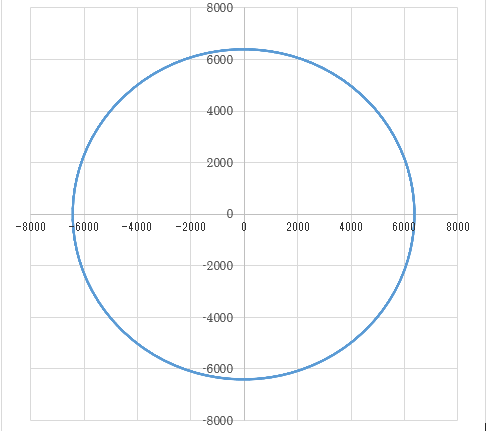
\includegraphics[height=7.5cm]{saijo/img/kiseki.PNG}
    \caption{物体の軌跡}
    % \label{sj-buttai-kiseki}
\end{figure}
座標$(6371.001,0)$を出発した物体が地球の周りを周回する様子を読み取ることができる。\par
求める速度を$v$とすると、円運動の運動方程式は
\begin{align}
    m\frac{v^2}{r} = mg
\end{align}
となる。$g=9.8\,\mathrm{m/s^2}$\,(重力加速度)とし、また、今回物体の質量$m$は1である(つまり今回の想定は地球上で$1\,\mathrm{kg}$の物体を投げた場合である)。よって速度の理論値は$v=\sqrt{gr}$より、約$7.9016\,\mathrm{km/s^2}$となる。これはシミュレーションによって求められた値と比較し約$0.5\%$の差である。この誤差は表\ref{tbl:sj-datadt}より、$dt$の値が大きすぎる、または小さすぎるためではないと考えられる。表3から読み取ると、初期位置に地表からある程度余裕をもった海抜を設定した場合のほうが理論値に近い速度が求められている。このことから、先ほどの誤差は、初期位置が地表から近すぎたことにより、小さな計算誤差によって地表に衝突したと判定された地点があったためであると考えられる。数値計算では有限の桁数で計算を打ち切っていることから、計算誤差は多少なりとも必ず発生していることは確かである。\par
以上の求められた値を、等速円運動の公式$v = \frac{2\pi r}{t}$ に代入すると、およそ正しい値(約1\%以内)となることと、理論値との誤差の量(約0.5\%)からも、およそ正しい値の速度が求められたと考えられる。


% - - - - - - - - - - - - - - - - - - -
% 参考文献
\sanko
\begin{enumerate}
\item 和田純夫, 「プリンキピアを読む」, 講談社.
\end{enumerate}
% - - - - - - - - - - - - - - - - - - -


% - - - - - - - - - - - - - - - - - - -
\section*{付録A 数値計算のプログラム}
% - - - - - - - - - - - - - - - - - - -
\begin{sjcode}
    Sub planet() '天体運行シミュレーション
'1定数の宣言
    Const dt As Single = 0.001 '時間の刻み
    Const Period As Single = 25000 '計算終了時刻
    Const Output_interval As Single = 1 '出力時間間隔
    
'2変数の宣言
    Dim t As Single
    Dim time_to_output As Single '次に出力する時刻
    Dim row_to_output As Single '出力する行
    Dim x As Single
    Dim y As Single
    Dim Vx As Single
    Dim Vy As Single
    Dim new_x As Single
    Dim new_y As Single
    Dim new_Vx As Single
    Dim new_Vy As Single
    Dim D As Single
    
'3初期条件の読み込み
    x = Range("B2")
    y = Range("C2")
    Vx = Range("D2")
    Vy = Range("E2")
    time_to_output = Output_interval
    row_to_output = 3

'4ループの実行
    For t = 0 To Period Step dt '軌道計算
        new_x = x + Vx * dt
        new_y = y + Vy * dt
        new_Vx = Vx + Ax(x, y) * dt
        new_Vy = Vy + Ay(x, y) * dt
        
        D = (x ^ 2 + y ^ 2) ^ 0.5
        
        x = new_x
        y = new_y
        Vx = new_Vx
        Vy = new_Vy
        
    If D < 6371 Then
        Cells(3, 7) = t
        Exit For
    End If
    
'5出力
    If t >= time_to_output Then
        Cells(row_to_output, 1) = t
        Cells(row_to_output, 2) = x
        Cells(row_to_output, 3) = y
        Cells(row_to_output, 4) = Vx
        Cells(row_to_output, 5) = Vy
'        Cells(row_to_output, 6) = Ax(x, y)
'        Cells(row_to_output, 7) = Ay(x, y)
        Cells(row_to_output, 6) = area_velocity(x, y, Vx, Vy) 'area_velocityを決める
        time_to_output = time_to_output + Output_interval
        row_to_output = row_to_output + 1 '行を降ろしていく
    End If
    
    Next t 'ここまでループ動作
        
End Sub

'位置から加速度を求める
    Function Ax(x As Single, y As Single) As Single
    Const G As Single = 6.67E-20 '万有引力定数
    Const M As Single = 6E+24 '地球質量
        Ax = -1 * G * M * x * (x ^ 2 + y ^ 2) ^ (-1.5)
    End Function

    Function Ay(x As Single, y As Single) As Single
    Const G As Single = 6.67E-20 '万有引力定数
    Const M As Single = 6E+24 '地球質量
        Ay = -1 * G * M * y * (x ^ 2 + y ^ 2) ^ (-1.5)
    End Function

'面積速度を求める
    Function area_velocity(x As Single, y As Single, v_x As Single, v_y As Single) As Single
       area_velocity = 0.5 * ((x ^ 2 + y ^ 2) * (v_x ^ 2 + v_y ^ 2) - (x * v_x + y * v_y) ^ 2)
    'area_velocityは決めた順通りに代入される
    End Function
\end{sjcode}


\end{document}
%
% ファイトだよ!
%